\documentclass[11pt]{article}
\usepackage[margin=1in]{geometry}
\usepackage{amsmath,amssymb,booktabs,graphicx,microtype,xcolor,url}
\usepackage{setspace}
\usepackage{placeins}
\emergencystretch=2em
\graphicspath{{figures/}}
\newcommand{\wq}{w_q}
\newcommand{\smin}{\sigma_{\min}}
\newcommand{\kappaJ}{\kappa(J)}
\title{Learning When Black-Hole Hair Is Observable:\\Physical Identifiability, Generalization, and Observable Complementarity}
\author{Ariadna Uxue Palomino Ylla\\Nagoya University, Nagoya, Japan\\\texttt{ariadnaepy@gmail.com}}
\date{}

\begin{document}
\maketitle

\begin{abstract}
High interpolation accuracy does not establish that physical parameters are
identifiable. We study this distinction in a controlled Kiselev black-hole
benchmark with a validated timelike-emitter and three-dimensional null-geodesic
shooting calculation. The forward analysis shows that ringdown is informative
for the deformation amplitude $k$, whereas photon geometry supplies an
independent response direction that resolves much of the state-parameter
$\wq$ degeneracy. Relative to ringdown alone, ringdown plus photon geometry
improves the grid-median minimum singular value by $4.54\times$ and the median
Jacobian condition number by $2.28\times$. In grouped physical interpolation,
the corresponding identifiable-$\wq$ normalized mean absolute error decreases
from 0.309 for ringdown to 0.087 for the combined features. Random splitting is
more optimistic, while four directional extrapolation tests are substantially
harder and split-conformal coverage falls under distribution shift. A uniform
161-phase audit gives a typical normalized prediction shift of
$9.48\times10^{-4}$ but exposes catastrophic extrapolation tails. A subsequent
targeted 321-phase audit resolves the remaining forward-feature comparisons,
yet frozen HGB and random-forest tail shifts exceed predeclared robustness
thresholds. Thus the physical complementarity result is supported, but inverse
estimator robustness remains conditional. This study is a theoretical
identifiability benchmark, not an observational constraint.
\end{abstract}

\section{Introduction}
Scientific inverse models can predict accurately for the wrong reason. Repeated
realizations of one physical system can leak across random partitions;
parameters can be locally degenerate even when observables respond strongly;
and a model can interpolate well while failing under extrapolation or small
numerical perturbations. These distinctions matter in black-hole spectroscopy,
where quasinormal frequencies encode compact-object properties but resolving
multiple physical effects remains difficult \cite{dreyer2004spectroscopy,berti2006spectroscopy,bhagwat2019overtones}.

Kiselev spacetimes provide a controlled two-parameter setting. They do not
stand in for a detector likelihood or a generic beyond-Kerr theory. Their value
here is methodological: exact loss of $\wq$ dependence at $k=0$ supplies a known
rank-deficient boundary, while nonzero $k$ permits direct comparison of forward
Jacobian geometry and inverse-learning behavior \cite{kiselev2003quintessence}.

The study complements rapid gravitational-wave inference based on neural
posterior estimation and normalizing flows
\cite{dax2021realtime,green2020autoregressive,gabbard2022cvae,cranmer2020frontier,papamakarios2021normalizing}.
Those methods address posterior computation; the present question is whether
the selected forward observables distinguish the parameters in the first
place. This distinction parallels structural and practical identifiability
analysis in dynamical inverse problems \cite{raue2009identifiability,villaverde2019identifiability}.

This work makes four contributions. It (i) evaluates inverse models with
leakage-aware random, grouped, and directional protocols; (ii) validates
timelike and null Kiselev geodesic shooting with explicit failure accounting;
(iii) quantifies physical Jacobian conditioning and observable
complementarity; and (iv) audits uncertainty, noise, learning curves, and
81--161--321 phase-resolution robustness under frozen estimators.

The central narrative rests on three distinctions: sensitivity is not
identifiability, interpolation is not generalization, and forward convergence
is not estimator robustness.

\section{Physical Model and Identifiability Framework}
The static spherical line element is
\begin{equation}
 ds^2=-f(r)dt^2+\frac{dr^2}{f(r)}+r^2d\Omega^2,
 \qquad f(r)=1-\frac{2M}{r}-\frac{k}{r^{1+3\wq}}.
\end{equation}
We use geometrized units with $M=1$. The dense historical synthetic domain and
the later 121-point physical shooting domain are distinct datasets and are not
mixed. Leading-eikonal ringdown features use the unstable circular null orbit,
with the known limitations of the geodesic--QNM correspondence kept explicit
\cite{cardoso2009geodesic,konoplya2017correspondence,palominoylla2026ringdown}.

For standardized observables $\tilde{\mathbf O}$ and parameters
$\boldsymbol\theta=(k,\wq)$, the local Jacobian is
\begin{equation}
 J_{ij}=\frac{\partial\tilde O_i}{\partial\theta_j}.
\end{equation}
Higher $\smin(J)$ and lower $\kappaJ=\sigma_{\max}/\smin$ are favorable. At
$k=0$, $f(r)$ is Schwarzschild for every $\wq$, so the $\wq$ Jacobian column
vanishes exactly. Nonzero rank away from that boundary does not by itself imply
practical recoverability at finite precision.

\begin{figure}[t]
\centering
\includegraphics[width=.82\linewidth]{learning_when_hair_is_observable_rank_aware.pdf}
\caption{Rank-aware identifiability boundary in the historical dense synthetic
domain. Exact $k=0$ rank loss is separated from finite-precision weak
identifiability.}
\label{fig:boundary}
\end{figure}

\section{Physical Geodesic Shooting and Numerical Validation}
The emitter follows the equatorial timelike Hamiltonian
\begin{equation}
 H=\tfrac12[-E^2/f+fp_r^2+L^2/r^2]=-\tfrac12.
\end{equation}
Its physical coordinate azimuth begins at apocentre:
$\phi=\pi$, $r=r_a$, $p_r=t=\tau=0$. Coordinate $\phi$ is not treated as a
radial anomaly; turning points are detected from $p_r=0$ and the radial
azimuthal period includes apsidal advance.

Photons are propagated in Cartesian spatial coordinates with covariant momentum
$\mathbf p$ and $p_t=-1$,
\begin{equation}
 H_\gamma=\tfrac12[-1/f+\mathbf p^2+(f-1)(\mathbf n\!\cdot\!\mathbf p)^2]=0.
\end{equation}
Two launch angles are solved so the direct branch reaches the observer plane.
The implementation reports failed phases rather than interpolating them or
substituting synthetic geodesic proxies. Photon momenta are projected onto the
static observer tetrad before sky angles are formed. Redshift uses
$1+z=\omega_{\rm emit}/\omega_{\rm obs}$, and direct arrival time is compared
with $\int(1+z)d\tau_{\rm emit}$ after removing one common additive constant.

In the Schwarzschild benchmark, all 161 phases succeed for both tested nominal
$\wq$ values, which agree because $k=0$. The independent radial benchmark
validates the turning-point period and apsidal advance. The physical 121-point
grid also preserves the Hamiltonian constraints and exact rank-loss boundary.

\begin{figure}[t]
\centering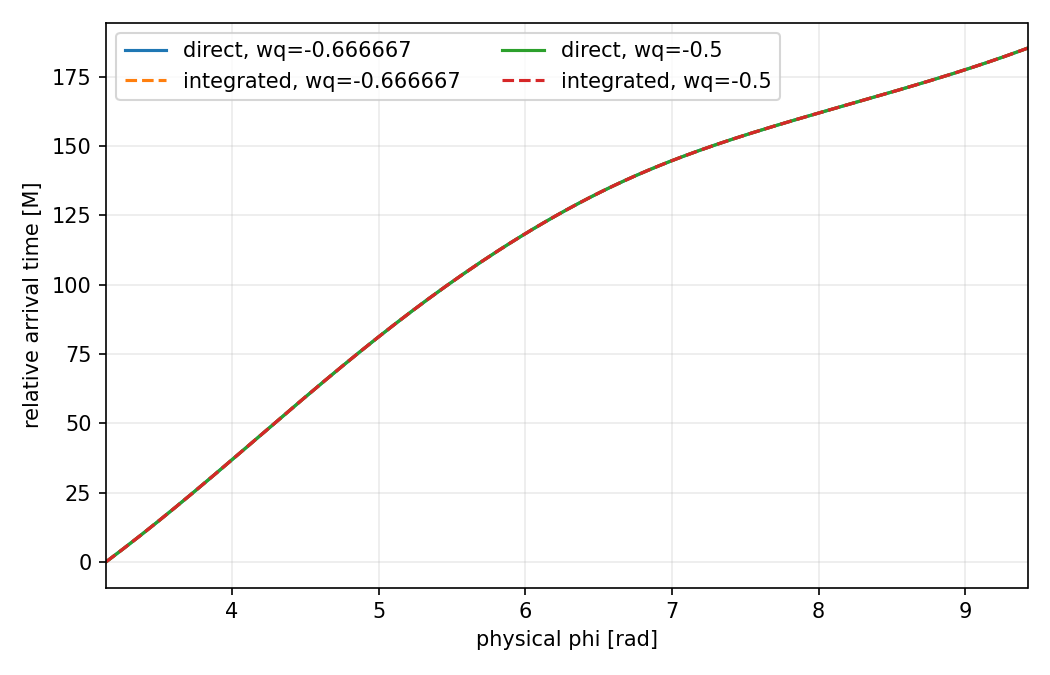
\includegraphics[width=.96\linewidth]{physical_schwarzschild_arrival_validation.png}
\caption{Schwarzschild shooting validation. Physical phase begins at
$\phi=\pi$ at apocentre. Direct arrival time and the integrated-redshift curve
share only the first-phase additive constant.}
\label{fig:schwarzschild}
\end{figure}

\section{Physical Observable Complementarity}
A large response can reveal that the spacetime changed without revealing which
parameter caused the change. Timing and redshift responses are often large but
nearly collinear in parameter space. Photon geometry rotates the sensitivity
direction and therefore contributes information that ringdown lacks.

\begin{figure}[t]
\centering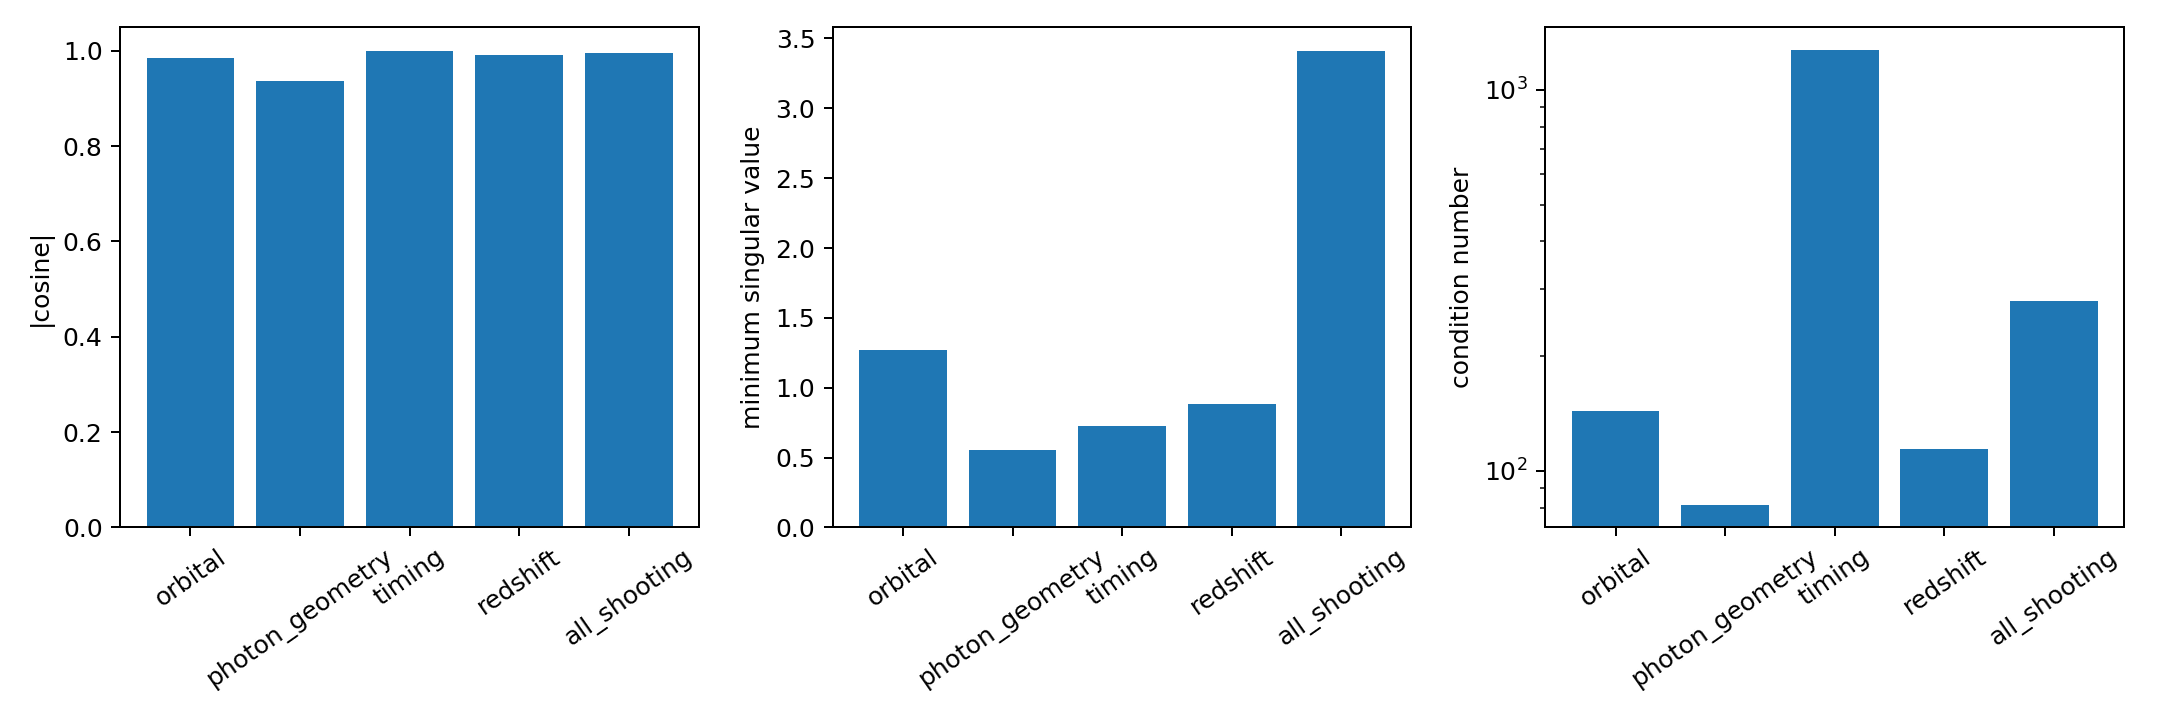
\includegraphics[width=.94\linewidth]{physical_local_sensitivity_comparison.png}
\caption{Local standardized sensitivity diagnostics. Higher minimum singular
value and lower condition number are better; response magnitude alone does not
establish parameter separation.}
\label{fig:local}
\end{figure}

Across the accepted physical grid, ringdown plus photon geometry improves the
median $\smin$ by $4.5429\times$ and the median condition number by
$2.2819\times$ relative to ringdown alone. The medians for the combined set are
$\smin=1.2326$ and $\kappaJ=4.0731$. Ringdown plus all shooting has
$\smin=1.5312$ and $\kappaJ=4.4974$: adding more responsive summaries can raise
$\smin$ without producing the best conditioning.

\begin{figure}[t]
\centering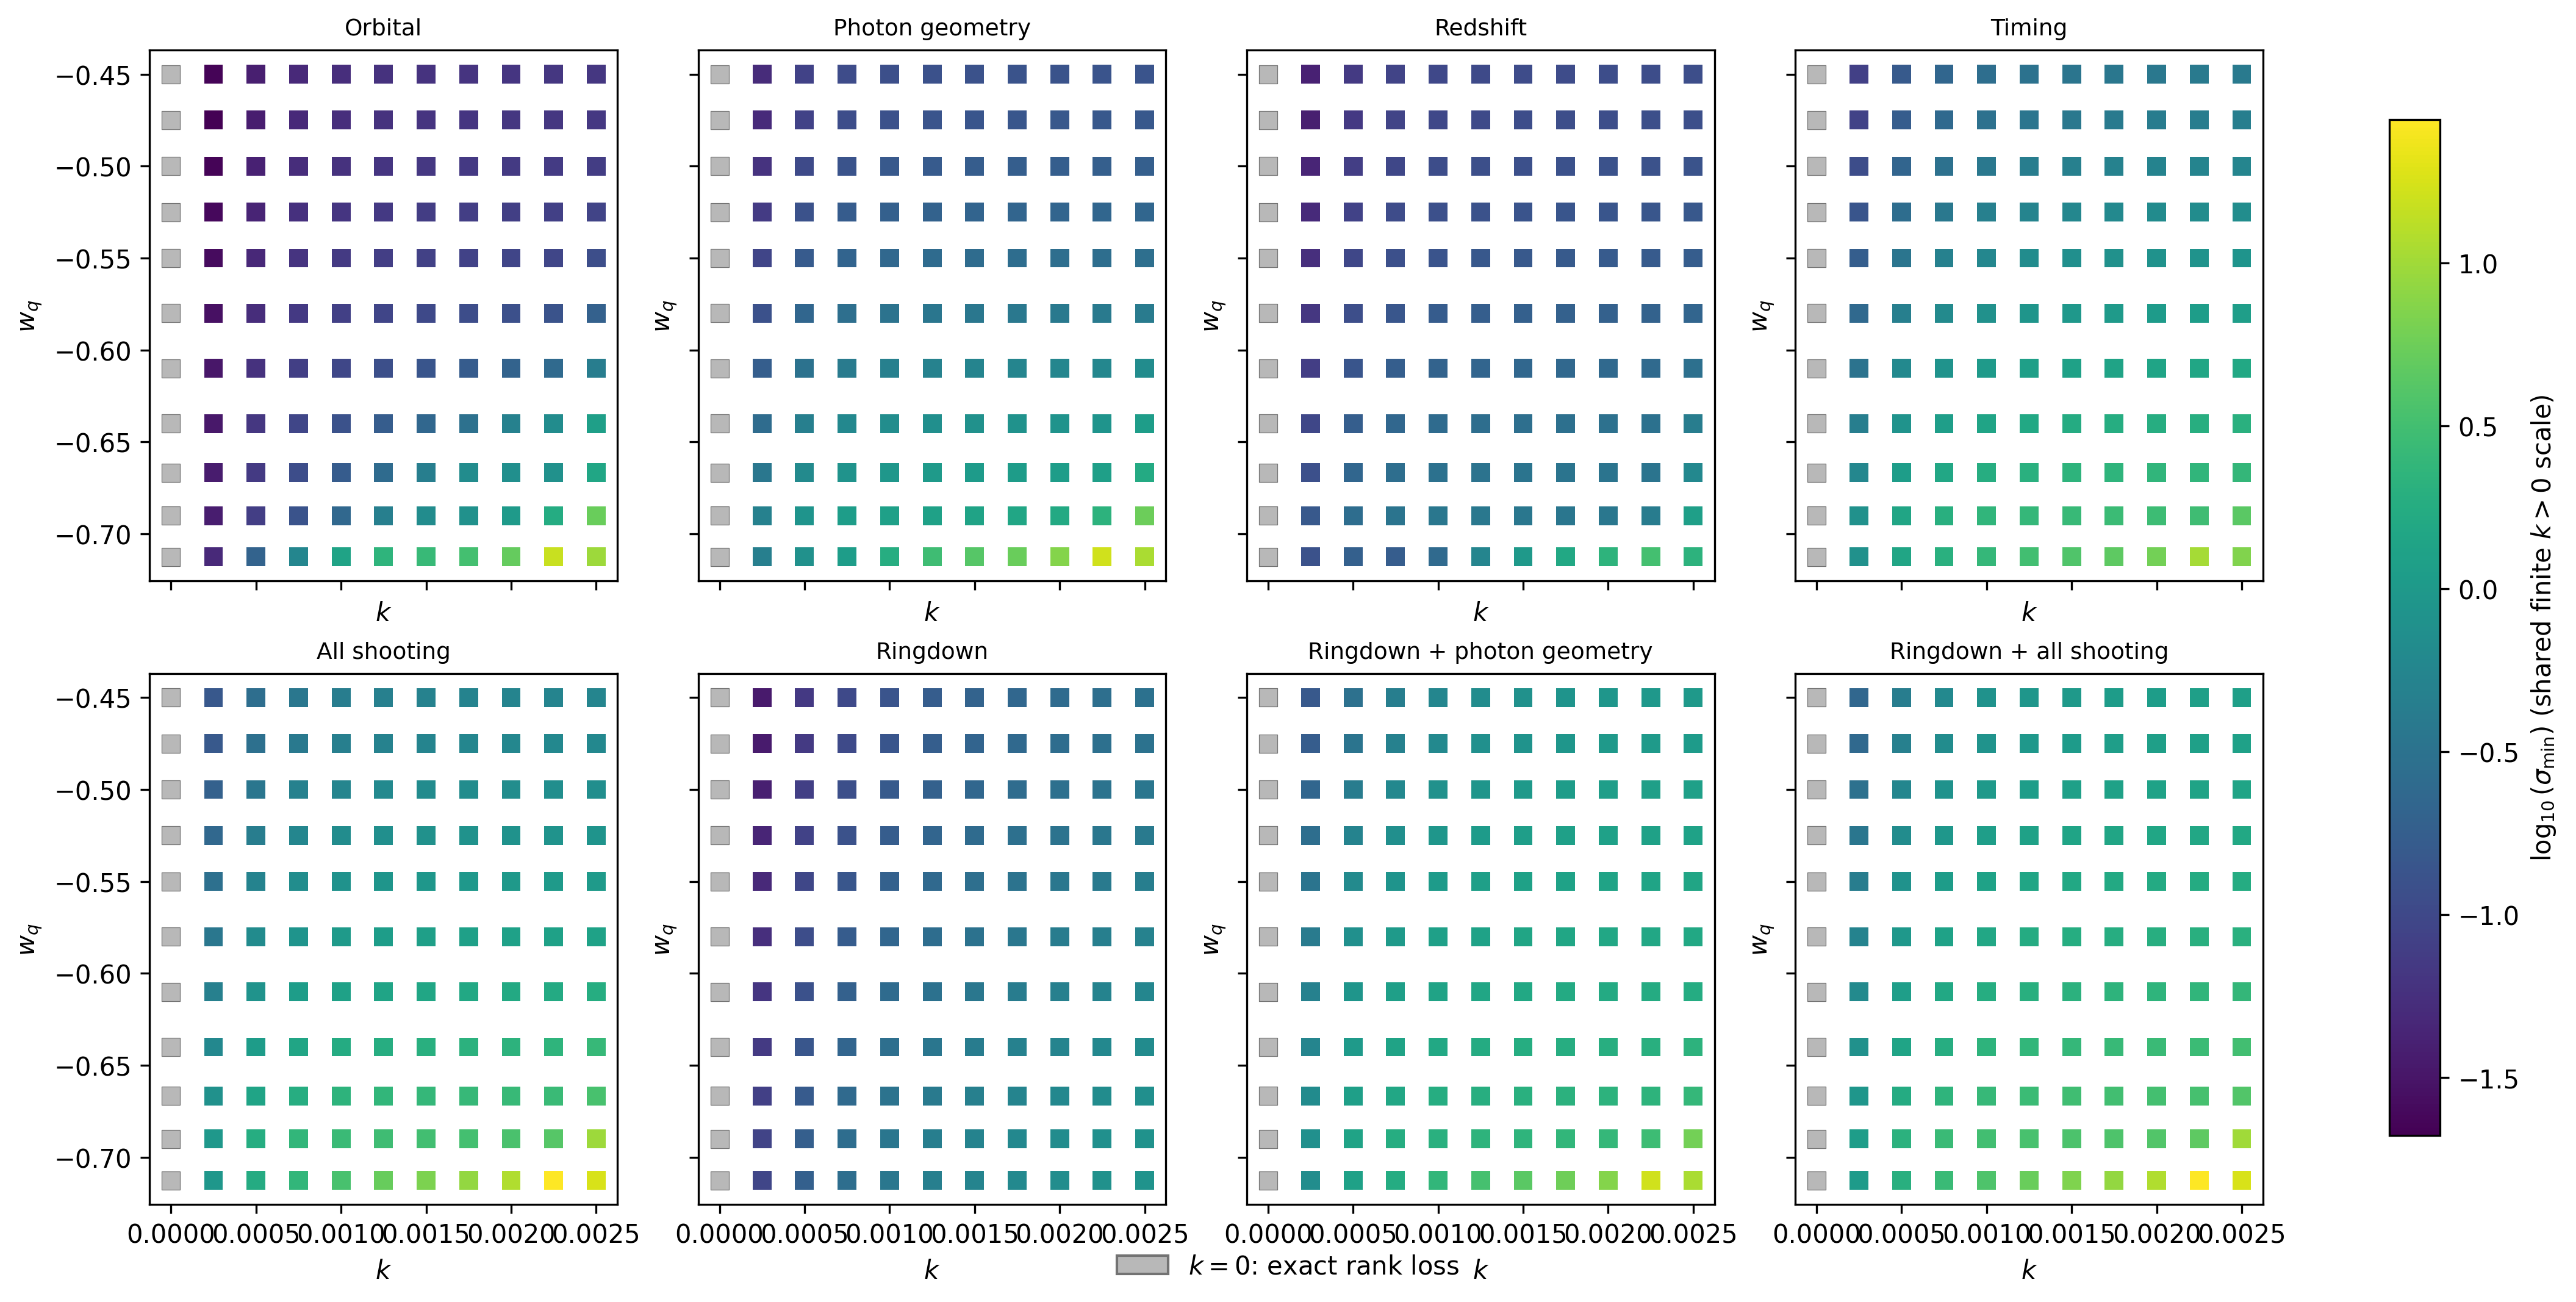
\includegraphics[width=.98\linewidth]{physical_grid_minimum_singular_value.png}
\caption{Grid maps of $\log_{10}\smin$ with exact $k=0$ rank-loss points
masked. Missing or invalid values are not interpolated, and all panels use one
finite-$k$ color scale.}
\label{fig:grid}
\end{figure}

\begin{figure}[t]
\centering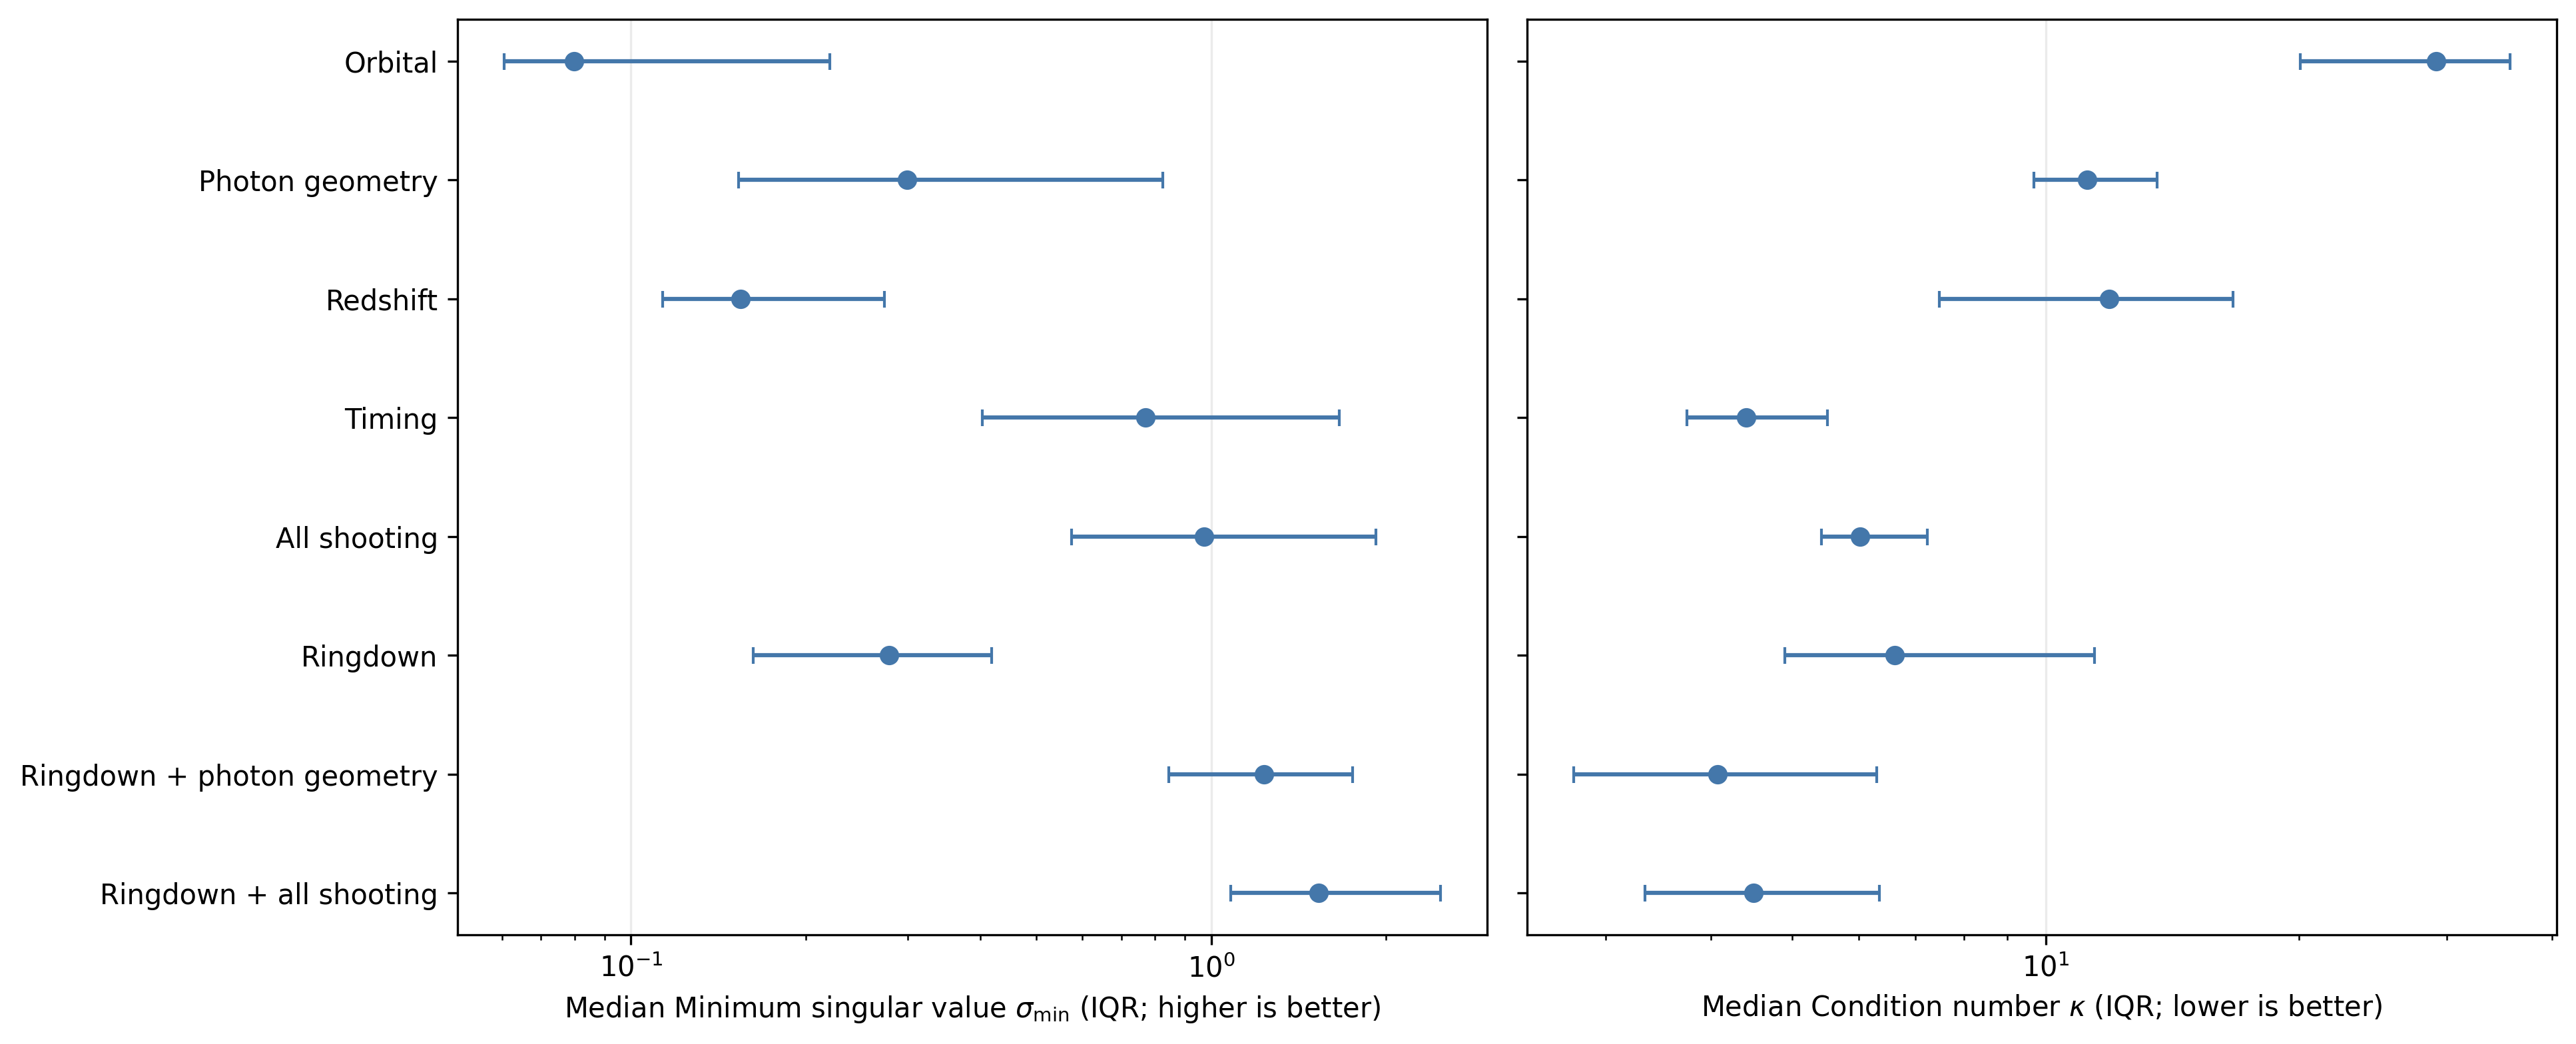
\includegraphics[width=.98\linewidth]{physical_observable_complementarity.png}
\caption{Grid-wide median and interquartile summaries of $\smin$ and condition
number. Photon geometry provides the clearest complement to ringdown.}
\label{fig:complementarity}
\end{figure}

\section{Leakage-Aware Inverse-Learning Protocols}
Five primary feature sets are ordered consistently: ringdown, photon geometry,
all shooting, ringdown plus photon geometry, and ringdown plus all shooting.
Here photon geometry and the other integrated quantities are physical shooting
observables, distinct from the historical synthetic geodesic proxies.
Models are histogram gradient boosting (HGB), random forest (RF), and a
target-scaled multilayer perceptron (MLP) \cite{breiman2001random,friedman2001greedy,pedregosa2011scikit}.
The protocols are random interpolation, two blocked $3\times3$ grouped physical
layouts, and four directional extrapolation tests. All nominal $k=0$ records
are retained and flagged, but ordinary $\wq$ error excludes them because $\wq$
is exactly non-identifiable there.

Normalized mean absolute error divides MAE by the full target span. Split-
conformal intervals target 90\% coverage and are interpreted under their
exchangeability assumptions \cite{vovk2005conformal,tibshirani2019covariate,angelopoulos2021guide}.
Feature-noise scales and every preprocessing transform are learned on training
folds. The 81-to-161 and targeted 161-to-321 comparisons apply archived frozen
estimators; they do not retrain on higher-resolution test features.

\section{Inverse-Learning Results}
Random splitting is optimistic. For HGB, RF, and MLP considered together,
random ringdown NMAE is 0.0361/0.1688 for $k$/identifiable $\wq$, while grouped
ringdown is 0.0485/0.3093. Ringdown plus photon geometry gives grouped
0.0457/0.0875, with the $\wq$ improvement reproduced independently in both
tree families. Directional extrapolation remains harder: the combined set has
aggregate NMAE 0.1305/0.2012.

\begin{figure}[t]
\centering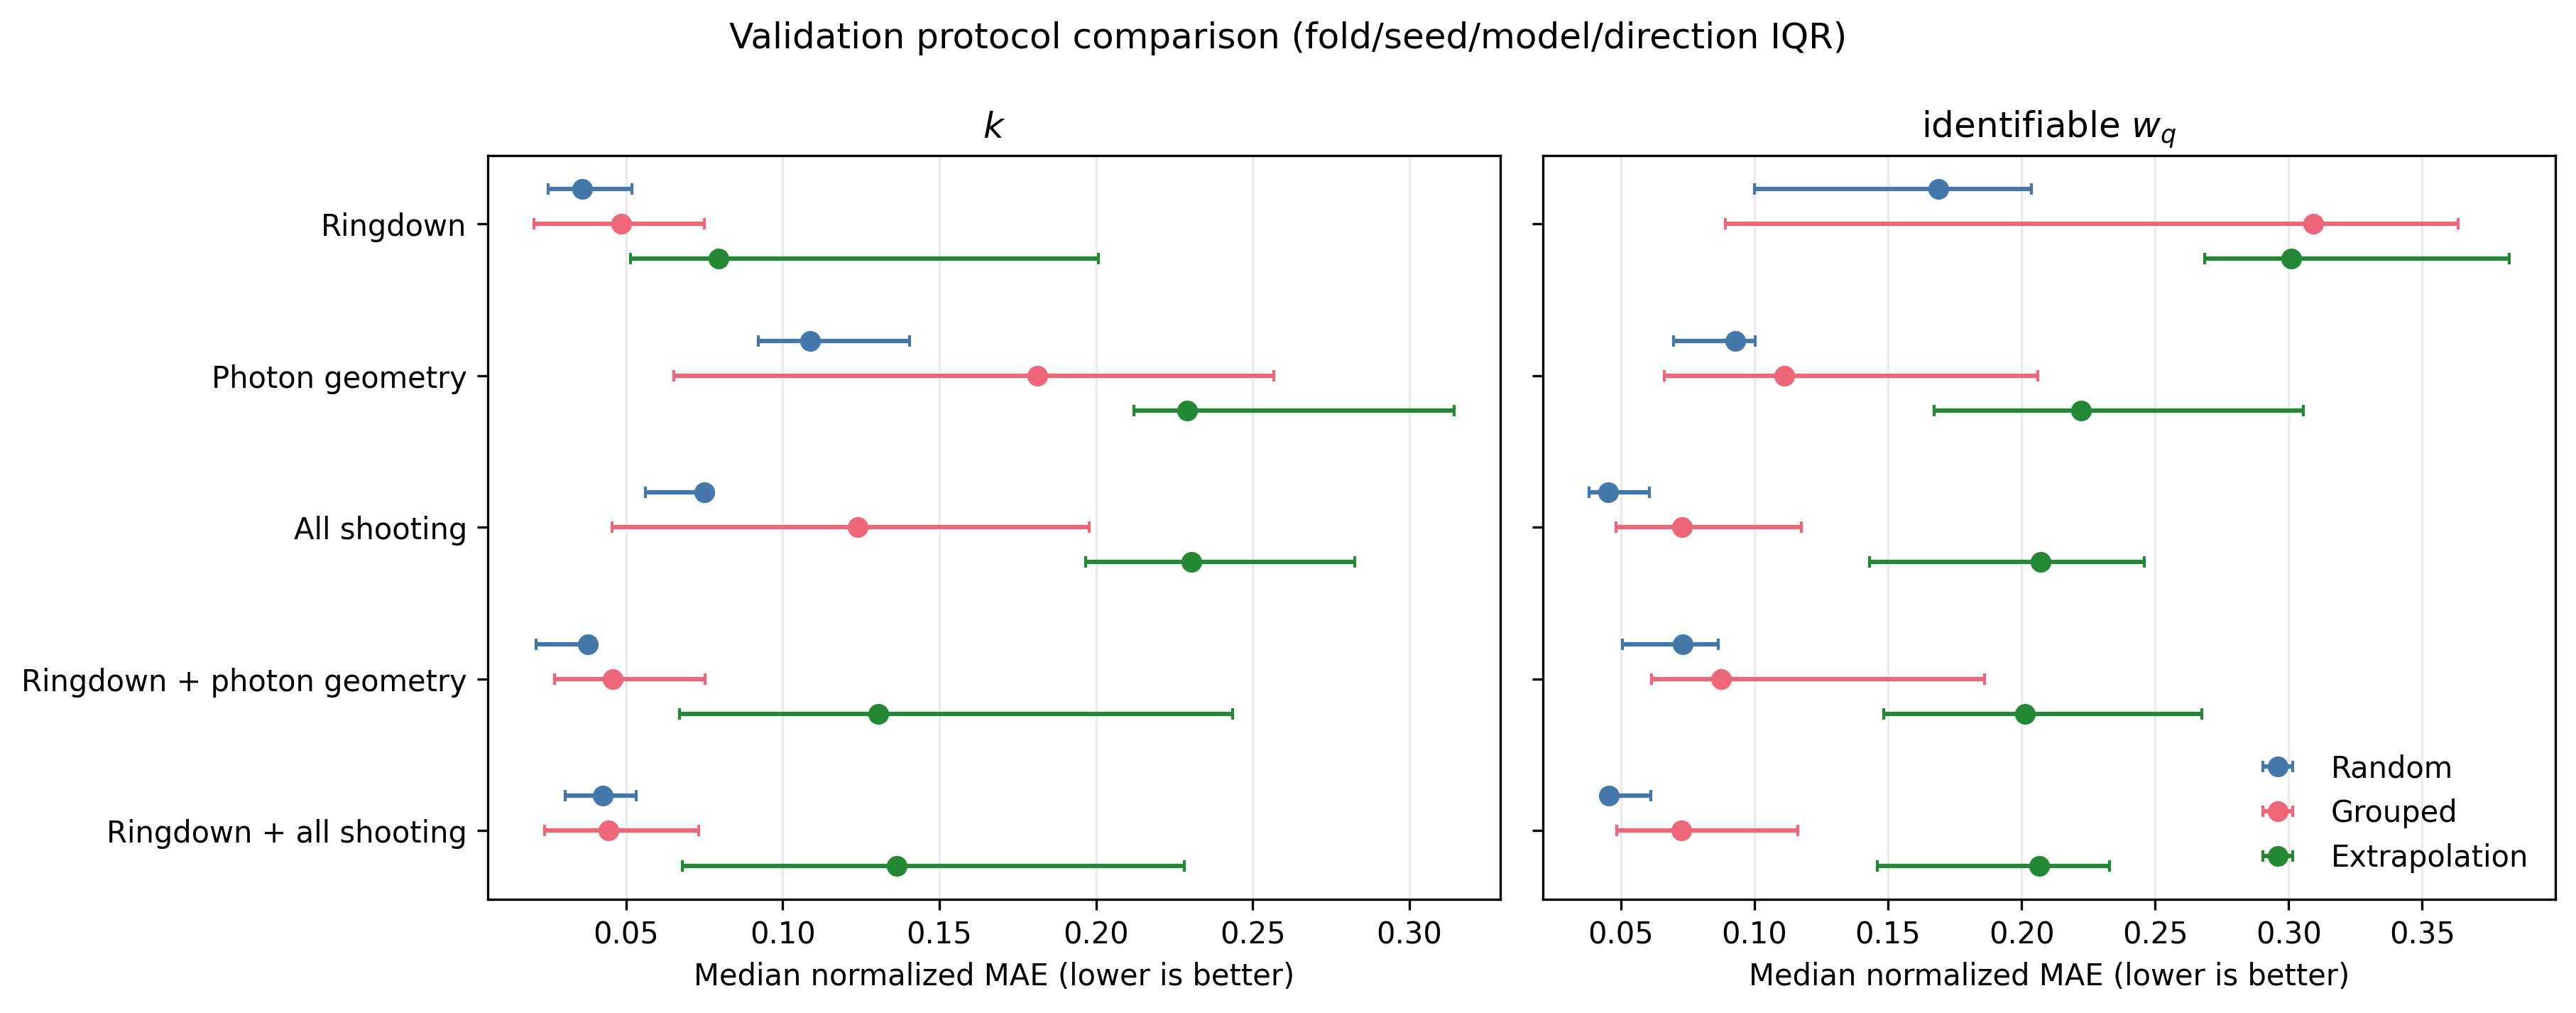
\includegraphics[width=.98\linewidth]{physical_ml_protocol_comparison.png}
\caption{Median NMAE for the five primary feature sets under random, grouped
physical interpolation, and directional extrapolation. Directions remain
separate in the machine-readable source before aggregation.}
\label{fig:protocols}
\end{figure}

Conditioning and coverage explain different aspects of error. In the error
model, standardized training distance has estimate 0.330, extrapolation status
0.276, and log condition number 0.197. Physical conditioning generally agrees
with grouped tree-based $\wq$ performance, but it does not perfectly rank every
model, target, or protocol. The MLP supplies a counterexample: it can have
reasonable central metrics while producing catastrophic directional tails.

\begin{figure}[t]
\centering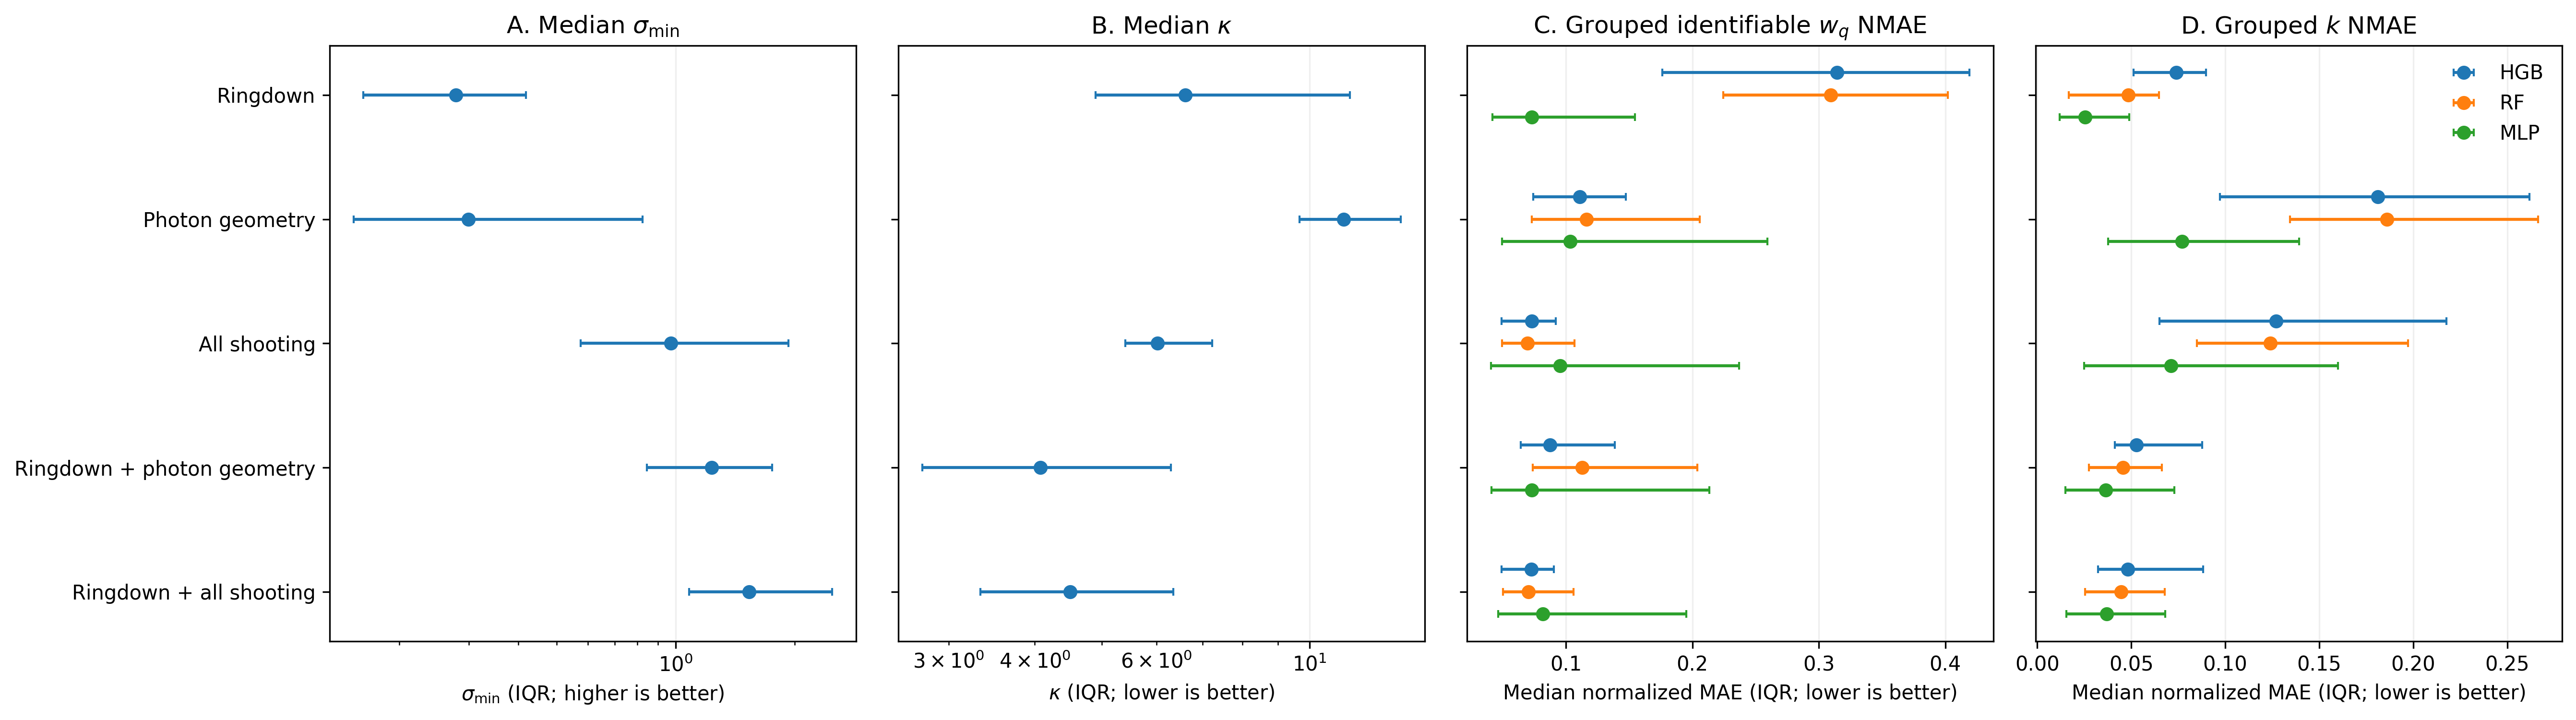
\includegraphics[width=.98\linewidth]{physical_ml_vs_jacobian_complementarity.png}
\caption{Aligned physical and empirical diagnostics: median minimum singular
value, median condition number, grouped identifiable-$\wq$ NMAE, and grouped
$k$ NMAE. Exact statistics and the feature order are shared across panels.}
\label{fig:mljac}
\end{figure}

Nominal 90\% conformal coverage is 0.892/0.965 for random $k/\wq$, but falls to
0.722/0.851 under grouped interpolation and 0.509/0.660 under extrapolation.
This is empirical coverage under shift, not a retained finite-sample guarantee.

\begin{figure}[t]
\centering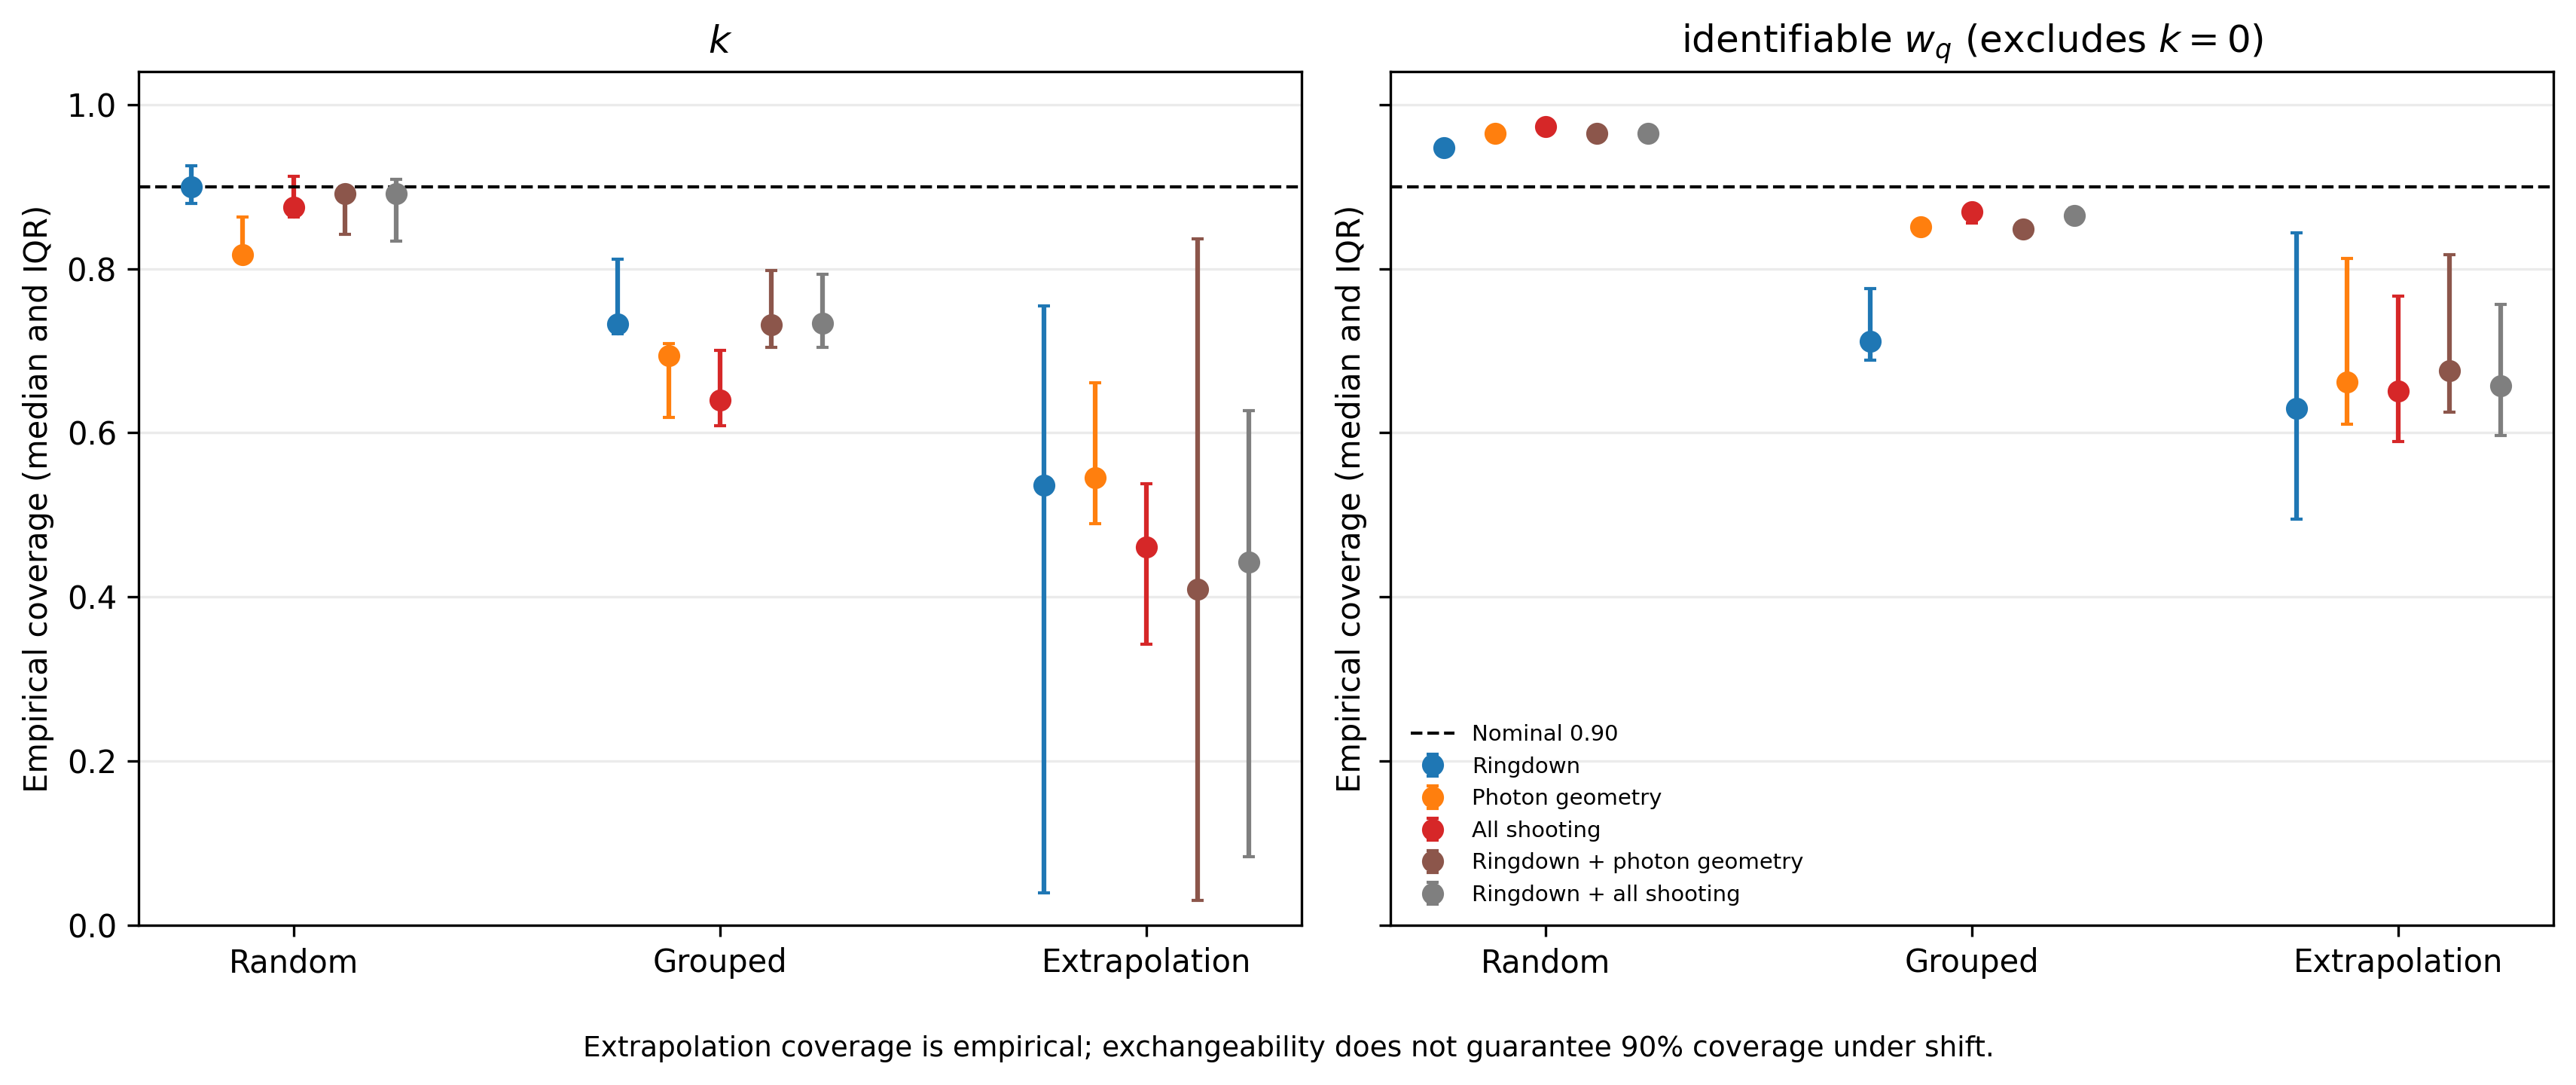
\includegraphics[width=.96\linewidth]{physical_ml_uncertainty_calibration.png}
\caption{Empirical 90\% split-conformal coverage by target and protocol.
Ordinary $\wq$ coverage excludes $k=0$; extrapolation coverage is not
guaranteed under distribution shift.}
\label{fig:coverage}
\end{figure}

\section{Numerical Convergence and Estimator Robustness}
The uniform 161-phase study completes all 121 physical points. From 9317
feature--point comparisons, 240 are unresolved under the frozen criterion;
the median normalized feature change is $7.908\times10^{-4}$ and the maximum is
0.08069. Across frozen scored predictions, the median normalized shift is
$9.482\times10^{-4}$ and the 95th percentile is 0.02606. The median aggregate
NMAE change is $6.880\times10^{-4}$, but the maximum is 16.8497 because of
un-clipped MLP directional extrapolation outliers.

The targeted 321-phase audit selects 35 points deterministically before reading
their 321-phase outcomes. All complete. Median and 95th-percentile normalized
161-to-321 feature changes are $1.963\times10^{-4}$ and $7.234\times10^{-3}$;
no comparison remains unresolved, ringdown is exactly unchanged, and Jacobian
rank is preserved. Forward convergence therefore passes.

\begin{figure}[t]
\centering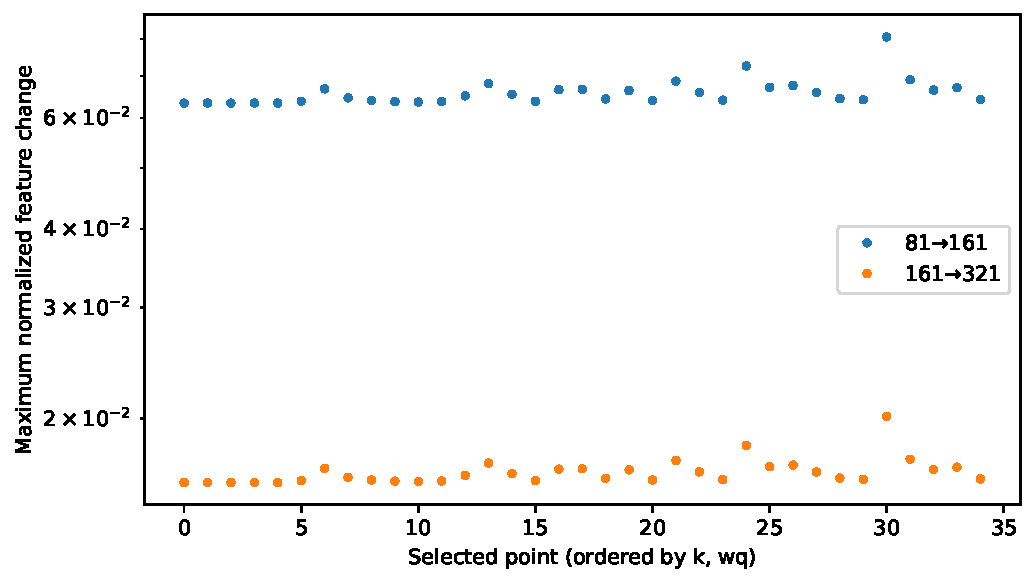
\includegraphics[width=.96\linewidth]{resolution_robustness.pdf}
\caption{Targeted pointwise maximum normalized feature changes from 81 to 161
and 161 to 321 phases. The 321-phase audit resolves the forward-feature
criterion but does not by itself certify inverse estimators.}
\label{fig:resolution}
\end{figure}

Frozen trees remain tail-sensitive: HGB and RF 95th-percentile normalized
shifts are 0.08122 and 0.08509, and their largest identifiable-$\wq$ shifts are
0.30593 and 0.27053. Their median shifts are zero because many tree predictions do
not cross a split threshold. The predeclared perturbation ensembles and fixed
Extra Trees smoother do not pass all stability and grouped-performance
criteria. Of 410 catastrophic MLP records, 409 are already catastrophic at 161
phases, none is materially worsened by the 321-phase substitution, 63 reach the
iteration limit, and no numerical overflow is detected. The decision is
Outcome B: the forward map converges, but estimator robustness does not.

Typical predictions are stable, but the tails are not. The earlier MLP maxima
are not representative of every estimator, while the targeted tree failures
show that the remaining issue also cannot be attributed solely to the MLP.
Journal readiness remains conditional.

\section{Discussion}
Jacobian conditioning answers whether nearby parameter directions are separated
by the chosen observables. Training distance answers whether a fitted estimator
has support where it is evaluated. Neither statistic subsumes the other.
Consequently, $\smin$ can predict broad observable-set ordering without ranking
every empirical model or protocol.

Tree ensembles are piecewise and can show zero median response followed by
large split-crossing tails. The MLP is smoother under the targeted feature
substitution but extrapolates to physically unreasonable values in archived
directional tests. These mechanisms are estimator-specific manifestations of a
general scientific-ML risk: a converged forward simulator does not ensure a
stable inverse surrogate \cite{ovadia2019uncertainty,koh2021wilds,psaros2023uq}.

What is specific to Kiselev is the metric deformation and exact $k=0$ loss of
$\wq$. What may generalize is the workflow: establish forward rank, seek
complementary observables, partition by physical systems, test directional
shift, and perturb frozen estimators at independently measured numerical scales.

\section{Limitations}
The ringdown model is leading-eikonal rather than a dedicated finite-$\ell$
perturbative spectrum. The spacetime is static. Shooting includes only the
direct photon branch, a point emitter and point observer, and no radiative
transfer, detector response, secondary images, strain likelihood, calibration
error, or model discrepancy. The physical grid is finite. Historical proxy
results remain synthetic. Although the targeted audit resolves higher-harmonic
forward differences on its selected set, it is not a uniform 321-phase grid and
tree tail sensitivity persists. MLP extrapolation is unstable. The verdict is
therefore conditional, and no result is an observational constraint.

\section{Conclusion}
Physical complementarity is supported: ringdown constrains $k$, while photon
geometry supplies an independent direction needed for much of the $\wq$
recovery. Random interpolation overstates recoverability relative to grouped
and directional validation. Finally, numerical and distribution-shift audits
are necessary before confident inverse claims: the forward features can
converge while fitted estimators remain fragile. These conclusions motivate
robust inverse methods and broader physical modeling before observational use.

\clearpage
\appendix
\section{Historical Synthetic and Proxy Benchmark}
The original dense benchmark used leading-eikonal curves, training-fold PCA,
and synthetic geodesic proxies. Waveform-only RF achieved
$R^2(k)=0.8960$ and $R^2(\wq)=0.9587$; HGB with proxy augmentation achieved
0.9793 and 0.9891. The rank-aware classifier reached macro F1 0.9928 with a
57.6\% weak-identifiability fraction. PCA compressed correlated information; it
did not create a new physical response direction. These historical results
motivated the physical shooting study and are not substituted for it.

\section{Full Split Definitions}
Random splits partition parameter points before mode-level realization. Grouped
physical interpolation holds out blocks under both registered $3\times3$
layouts. Directional extrapolation separately holds high $k$, low $k$, high
$\wq$, and low $\wq$ sides. Calibration points are disjoint from training and
test points, and the archived assignments are reused exactly.

\section{Additional Model-Level Results}
HGB and RF reproduce the central grouped photon-geometry improvement for
identifiable $\wq$. The MLP is retained as a stress test rather than omitted:
its catastrophic errors are un-clipped and included in aggregate summaries.

\section{Four Directional Extrapolation Tests}
Directions are stored independently in the prediction tables before any median
summary. High-to-low and low-to-high tests differ in training support and cannot
be interpreted as interchangeable folds.

\section{Conformal Calibration and Rejection}
Split-conformal residual quantiles are fitted on calibration subsets. The
exchangeability guarantee applies to matching distributions; shifted coverage
is reported empirically. Rejection curves rank uncertainty but do not repair
distribution shift.

\section{Noise and Learning Curves}
Grouped one-percent feature noise yields ringdown-plus-photon-geometry NMAE
0.0699/0.0853 for $k/\wq$. Learning curves are still improving at 78 training
points, so data limitation remains part of the interpretation.

\section{Numerical-Validation Thresholds}
The 35-point 321-phase run takes 5318.2 s. Maximum hit, timelike-constraint,
null-constraint, and impact-parameter-drift errors are respectively
$7.0913\times10^{-8}$, $3.1303\times10^{-13}$,
$7.6214\times10^{-12}$, and $1.7932\times10^{-11}$.

\section{Uniform 161-Phase Convergence Audit}
All 121 points complete in 4473.2 s with zero failed points. The audit preserves
the exact $k=0$ boundary and uses no mixed-resolution row, interpolation, or
proxy substitution.

\section{MLP Extrapolation-Failure Audit}
The machine-readable table contains standardized input magnitude, hidden
activation magnitude, iteration status, overflow flag, training distance, and
resolution response for every catastrophic record. It distinguishes
optimization failure from extrapolation instability without clipping.

\FloatBarrier
\bibliographystyle{plain}
\bibliography{references}
\end{document}
